\documentclass{article}
% My first document using a professionnal editor!

\usepackage[T1]{fontenc}
\usepackage[french]{babel}

\usepackage{amsmath, amssymb}
\usepackage{listings}
\usepackage{graphicx}

\begin{document}
This is my first \LaTeX{} document with a spaces test and.

A new \ \ paragraph.

\tableofcontents
\listoffigures
\listoftables

\section{Titre}\label{section:titre}

Today is \today.

Let's  have a new textâ

\subsection{Text}\label{subsection:text}

\emph{test}
\textbf{test}
\texttt{test}
\textit{test}
\textsc{test}

\subsection{Sous-titre}\label{subsection:soustitre}
ce\-su\-re

The {\Large small} text is written in {\tiny big} and conversely;

\section{Titre 2}

\textbf{italic} is \texttt{written} in \textit{bold} and conversely.

\subsection{Références}

Titre: \ref{section:titre} \pageref{section:titre}

Titre/Text: \ref{subsection:text} \pageref{subsection:text}

Titre/Sous-titre: \ref{subsection:soustitre} \pageref{subsection:soustitre}

\subsection{Environment}

\begin{center}
Je suis centré!!!

Mon super tableau:
\begin{tabular}{|c|c|c|}
	\cline{2-3}
	\multicolumn{1}{c}{} & \multicolumn{2}{|c|}{OXO}\\
	\hline
	X & O & X\\
	\hline
	X & X & X\\
	\hline
	O & X & O\\
	\hline

	\label{table}
\end{tabular}
\end{center}

Le tableau plus haut était Table~\ref{tab:table}

\begin{itemize}
\item Premier
\item Deuxième
	\begin{itemize}
	\item Premier
	\item Deuxième
	\end{itemize}
\end{itemize}

\begin{enumerate}
\item Premier
\item Deuxième
	\begin{enumerate}
	\item Premier
	\item[(c)] Deuxième
	\end{enumerate}
\end{enumerate}


\begin{verbatim}
\ref{titre}
\end{verbatim}

Voici une référence: \verb|\ref{titre}|

$\sin^2x+\cos^2x=1$

\subsection{Figures}

\begin{figure}[ht]
\begin{center}
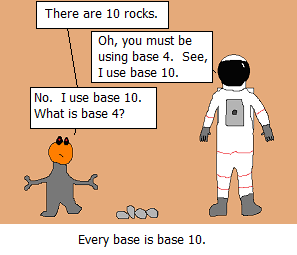
\includegraphics[width=0.5\textwidth]{EveryBaseIsBase10.png}
\end{center}
\caption{Une blague}
\label{fig:blague}
\end{figure}

N'oubliez pas figure~\ref{fig:blague}

\subsection{Mathématiques}

Soit $f'(x)+3f(x)=x^2+2x+4$;

Solution de l'équation homogène:
\begin{equation*}
	\begin{aligned}
	af(t)+bf'(t)+cf''(t)=0&\iff ake^{rt}+bkre^{rt}+ckr^2e^{rt}=0
		\\&\iff ke^{rt}(a+br+cr^2)=0
		\\&\implies \begin{cases}
			f_{\text{ESSM}}=k_1e^{r_1t}+k_2e^{r_2t}\text{ si }\Delta>0\\
			f_{\text{ESSM}}=ke^{rt}\text{ si }\Delta=0\\
			f_{\text{ESSM}}=k_1e^{r_1t}+k_2e^{r_2t}\text{ sinon}
		\end{cases}
	\end{aligned}
\end{equation*}

\subsection{Code}

\begin{lstlisting}[language=C]
#include <stdio.h>
#include <stdlib.h>

int main(void){
	printf("Hello world");

	return EXIT_SUCCESS;
}
\end{lstlisting}

\subsection{Includes}

\input{intro}
Thus, please refer to the beginning.

\end{document}